\subsubsection{Exercice}
The largest and smallest singular values for the system at different frequencies for the minimum phase model are visible on figure \ref{singvalue}.

\begin{figure}[h!b]
    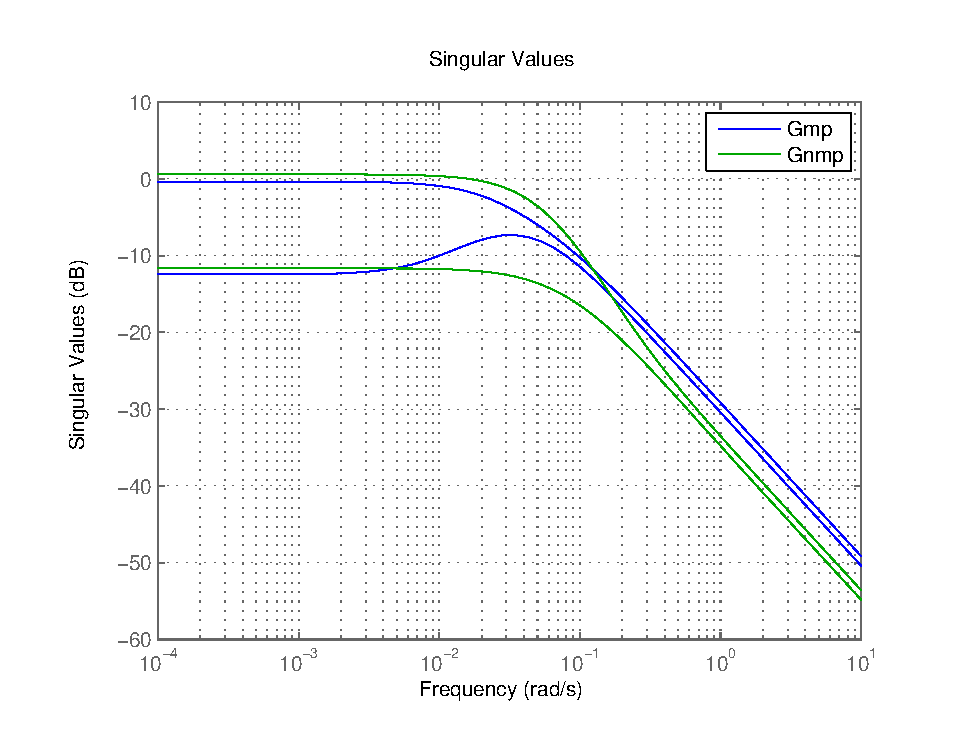
\includegraphics[width=\columnwidth]{fig/singvalue}
    \caption{$\underline{\sigma}(G(i\omega))$ and $\bar{\sigma}(G(i\omega))$ for the minimum phase model (blue) and the non-minimum phase model (green)}
    \label{singvalue}
\end{figure}

We have the following value for the $H_{\infty}$ norm of the systems:

$$\begin{array}{ccc}
    ||G||_{\infty,mp} =  .96
    & \text{ \textbf{and} } &
    ||G||_{\infty,nmp} = 1.1 
\end{array}
$$

